\section{Mass Index}
\label{sec:1ATR}

Mass Index wskaźnik jest pomocny w identyfikacji punktów zwrotnych, poprzez mierzenie odległości pomiędzy cenami maksymalnymi a minimalnymi. Według autora zmiana kierunku trendu następuje w momencie zaobserwowania tzw. wybrzuszenia zwrotnego, czyli wejścia wskaźnika ponad poziom 27 i następnie spadku poniżej 26,5. Wskaźnik nie identyfikuje jednak kierunku trendu, ustala jedynie punkt zwrotny. Sposób wyliczenia kolejnych wartości wskaźnika dla danego punktu w czasie przedstawia wzór \ref{wzor_3}.
\begin{equation}
Mass Index = \sum_{0}^{24} \left[\begin{array}{c} \frac{ EMA(H - L, 9)}{ EMA(EMA(H-L, 9), 9)}\end{array}\right]\\
\label{wzor_3}
\end{equation}

\noindent Sama interpretacja wskaźnika nie pozwala na wskazanie momentów w których mogą być zawierane konkretne transakcje (kopno/sprzedarz). W określeniu czy jest to sygnał kupna czy sprzedaży autor zaleca stosowanie 9- dniowej ekspotencjalnej średniej na wykresie notowań. Dlatego przyjeliśmy zasadę, która zakłada, że po wystąpieniu wybrzuszenia zwrotnego przyjmujemy jako sygnał kupna sytuację gdy wartość ceny zamknięcia przewyższa wartość 9- dniowej ekspotencjalnej średniej. Natomiast, gdy wartość ceny zamknięcia jest mniejsza od wartość 9- dniowej ekspotencjalnej średniej, to przyjmuje się taką sytuację za sygnał sprzedaży. Zostało to przedstawione na rysunku \ref{kupsprz2}. \\
\begin{figure}[h!]
\centering
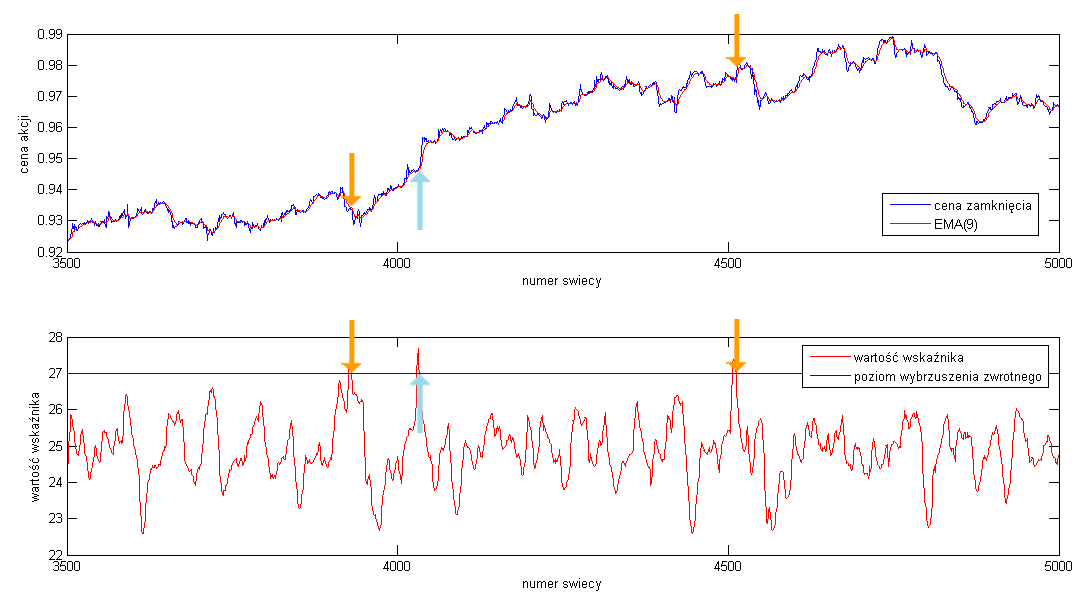
\includegraphics[width = \textwidth]{mi2.png}
\caption{Fragment przebiegu kursu akcji z naniesioną  9- dniową ekspotencjalną średnią (górny wykres) oraz odpowiadające jemu wartości wskaźnika indeksu masy wraz z sygnałami kupna --- zielone strzałki oraz sygnałami sprzedaży --- czerwone strzałki (dolny wykres)}
\label{kupsprz2}
\end{figure}
\FloatBarrier

\noindent Poniższy listing przedstawia zaimplementowaną w środowisku MATLAB strategię wykorzystującą opisywany wskaźnik.
\begin{scriptsize}
\begin{lstlisting}
bestiL = 0;
bestiS = 0;
HL = C(:,2) - C(:,3); % różnica H - L
kon=candlesCount-1;
MI = zeros(candlesCount,1);
HLaverage = ema(HL,9);
EMA2 = HLaverage(9:end) ./ ema(HLaverage(9:end),9);
for i = 41:kon-16
    MI(i) = sum(EMA2(i-24:i));
end
Caverages = ema(C(:,4),9);

sumR=zeros(1,candlesCount);
R=zeros(1,candlesCount);
pocz=50;
iL=0; %liczba otwieranych pozycji kupna
iS=0; %liczba otwieranych pozycji sprzedarzy
lastCandle = kon-16;
recordReturn=0;  %rekord zysku
recordDrawdown=0;  %rekord obsuniecia
LastPos = 0;
pic1 = false;

for i=pocz:lastCandle
    
    if pic1 == false && MI(i) > 27 % warunek wystąpienia wybrzuszenia zwrotnego
        pic1 = true;
    end
    if pic1 == true && MI(i) < 26.5 % warunek zawarcia transakcji
        if C(i,4) > Caverages(i) % warunek kupna
            R(i)= -C(i+1,4)-LastPos-spread; % zamknięcie S
            LastPos = C(i+1,1); % otwarcie L
            iL=iL+1;
        elseif C(i,4) < Caverages(i) % warunek sprzedaży
            R(i)=C(i+1,4)-LastPos-spread; % zamknięcie L
            LastPos = C(i+1,1); % otwarcie S
            iS=iS+1;
        end
        pic1 = false;
    end
    sumR(i)= sum(R(pocz:i));  %krzywa narastania kapitału
    
    if sumR(i)>recordReturn
        recordReturn=sumR(i);
    end
    
    if sumR(i)-recordReturn<recordDrawdown
        recordDrawdown=sumR(i)-recordReturn;  %obsuniecie maksymalne
    end
end

%wyniki końcowe
sumReturn=sumR(lastCandle);
Calmar=-sumReturn/recordDrawdown;  %wskaznik Calmara
\end{lstlisting}
\end{scriptsize}


Na podstawie zebranych informacji dotyczących wskaźnika $Mass Index$ utworzono prostą strategię inwestycyjną bazującą na regule: jeśli wystąpi wybrzuszenie zwrotne oraz wartość ceny zamknięcia przewyższy wartość 9- dniowej ekspotencjalnej średniej, to otwierana jest pozycja długa ($L$), a zamknięta pozycja krótka ($S$), która została wcześniej otwarta . Natomiast, gdy wartość ceny zamknięcia będzie mniejsza od wartość 9- dniowej ekspotencjalnej średniej, to otwarta zostanie pozycja krótka ($S$), a zamknięta długa. Badania zostały przeprowadzone na parze walutowej $CADCHF$ (szereg czasowy przedstawiony na rysunku \ref{rys2}). \\

Ze względu na to iż wszystkie parametry wzoru są arbitralnie ustawione, to zbiór danych (świec) nie został podzielony na dwie części: uczącą i testującą ($40\%$ całości). Na całym zbiorze danych weryfikowano skuteczność strategii. \\


\newpage
\noindent \textbf{I Wyniki badań.}\\
\begin{figure}[h!]
\centering
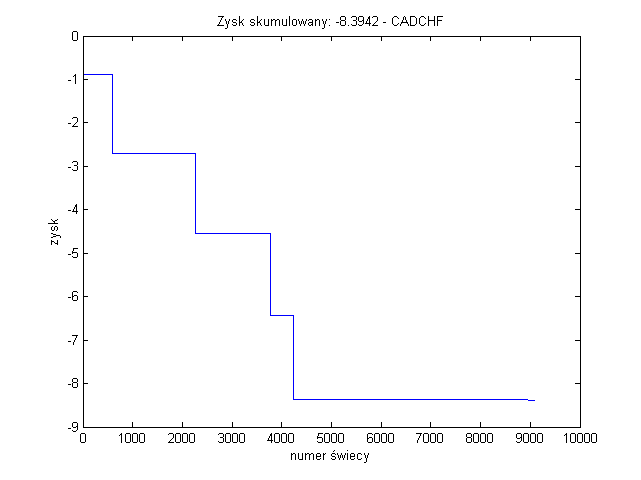
\includegraphics[width = 0.6\textwidth]{MI_CADCHF_S4LS.png}
\caption{Zysk skumulowany CADCHF na okresie testowym przy maksymalizacji według zysku}
\end{figure}
\FloatBarrier
\begin{verbatim}
OKRES WALIDUJĄCY
Zysk skumulowany:     -8.3942
Calmar:     -1
Liczba otwartych pozycji długich:     5
Liczba otwartych pozycji krótkich:     3
\end{verbatim}
%
